\documentclass[11pt,a4paper]{article}

% ---------------------------------------------------------------------------
% Packages
% ---------------------------------------------------------------------------
\usepackage[margin=1in]{geometry}
\usepackage{times}
\usepackage{amsmath,amssymb,amsfonts}
\usepackage{booktabs}
\usepackage{graphicx}
\usepackage{xcolor}
\usepackage{hyperref}
\usepackage{microtype}
\usepackage{setspace}
\usepackage{caption}
\usepackage{subcaption}
\usepackage{enumitem}
\usepackage[numbers,sort&compress]{natbib}

\hypersetup{
  colorlinks=true,
  linkcolor=black,
  citecolor=blue!50!black,
  urlcolor=blue!50!black
}

\setstretch{1.08}
\captionsetup{font=small,labelfont=bf}

% ---------------------------------------------------------------------------
% Title
% ---------------------------------------------------------------------------
\title{%
  PairFold: Fast Local Backbone Generation via\\
  Calibrated Fragment Assembly, Look-Ahead Backtracking,\\
  and Lever-Effect Torsion Relaxation%
}

\author{%
  PairFold Development Team\\
  \texttt{e:\textbackslash Programing\textbackslash Protein} --- Local Computational Biology Project\\
  \small Correspondence regarding software and benchmarks: project repository
}

\date{\today}

\begin{document}
\maketitle

% ===========================================================================
\begin{abstract}
High-accuracy structure predictors such as AlphaFold~2 have transformed structural biology, yet their memory footprint and quadratic attention costs remain limiting for interactive design, long-sequence screening, and deployment on commodity GPUs.
We present \textbf{PairFold}, a deliberately local alternative that predicts backbone dihedral angles $(\phi,\psi)$ for short peptides of length $2$--$5$ with a compact Transformer trained on high-resolution PDB fragments, then assembles longer chains with near-linear ($O(N)$) procedures.
The inference stack combines dynamic-programming segmentation that maximises calibrated fragment confidence, multi-window overlap consensus via circular means, secondary-structure block freezing, and a clash-aware look-ahead backtracking assembler with local $\phi/\psi$ perturbation ($\pm 1^\circ$--$5^\circ$) to mitigate cumulative ``lever-arm'' error.
Confidence is sharpened by softmax temperature scaling ($T{=}0.55$) with a disorder-aware prior.
On five standard small domains (1A8O, 1CRN, 2GB1, 1UBQ, 3GB1), PairFold with the contact head yields Kabsch-aligned C$\alpha$ RMSD between $13.12$\,\AA\ and $19.38$\,\AA\ (mean $17.17$\,\AA) with wall-clock times of $14.4$--$45.7$\,s (mean $27.9$\,s) on a single consumer GPU.
Look-ahead assembly, predicted long-range contact anchors, and post-secondary-structure lever polish improve local steric plausibility and reduce global RMSD relative to the prior local-only baseline (mean $18.50$\,\AA), while remaining far from AlphaFold-level tertiary accuracy.
PairFold is therefore best understood as a fast, low-resource backbone generator that now includes a lightweight long-range contact prior, not as a competitor to end-to-end folding networks.
\end{abstract}

\noindent\textbf{Keywords:}
protein backbone prediction;
dihedral angles;
contact prediction;
fragment assembly;
temperature scaling;
steric clash avoidance;
look-ahead backtracking;
computational biophysics.

% ===========================================================================
\section{Introduction}
% ===========================================================================

Protein structure prediction has entered a new regime with deep learning systems that integrate multiple-sequence alignments, pair representations, and iterative structure modules~\citep{jumper2021alphafold,senior2020alphafold}.
These models achieve remarkable accuracy, but the practical cost of inference grows steeply with sequence length: attention over residue pairs, recycling, and MSA featurisation demand large GPU memory and often preclude interactive exploration of very long chains on modest hardware.

Complementary lines of work emphasise speed or locality.
Language-model predictors such as ESMFold~\citep{lin2023evolutionary} remove MSA dependence at the expense of still-substantial model size.
Classical fragment-assembly approaches~\citep{simons1997assembly,rohl2004rosetta} and dihedral-angle representations~\citep{ramachandran1963stereochemistry} remain attractive when the scientific goal is \emph{local} backbone geometry rather than full tertiary fold recovery---for example, in educational tools, rapid prototyping of helix/sheet segments, or streaming visualisation of chains far beyond typical AlphaFold session lengths.

\textbf{PairFold} occupies this niche.
It trains a small Transformer exclusively on contiguous PDB fragments of length $2$--$5$, maps each fragment to $(\phi,\psi)$, and reconstructs longer proteins by segmentation and assembly.
The design goals are explicit:
\begin{enumerate}[leftmargin=1.5em,itemsep=0.25em]
  \item \textbf{Near-linear scaling} for queries up to tens of thousands of residues at the angle level;
  \item \textbf{Calibrated confidence} usable for dynamic-programming segmentation;
  \item \textbf{Physics-informed post-processing} (steric clashes, secondary-structure constraints, and lever-effect relaxation) without a full force field;
  \item \textbf{Honest scope}: PairFold does \emph{not} claim AlphaFold-competitive global RMSD.
\end{enumerate}

This paper describes the full method as implemented in the PairFold codebase, reports exact benchmark timings and C$\alpha$ RMSD on five public structures, and discusses the speed--accuracy trade-off introduced by look-ahead backtracking and torsion relaxation.

% ===========================================================================
\section{Methodology}
% ===========================================================================

\subsection{Dihedral representation and fragment network}
\label{sec:network}

Each residue $i$ is parameterised by backbone torsions $(\phi_i,\psi_i)$.
Cartesian C$\alpha$ (and optional full-backbone) coordinates are obtained by sequential placement with ideal peptide bond geometry~\citep{engh1991accurate}, as implemented in \texttt{dihedrals\_to\_ca} / \texttt{build\_backbone}.

The learned model, \texttt{FragmentTorsionNet}, is a Pre-LN Transformer encoder with
$d_{\mathrm{model}}{=}160$, $4$ heads, $4$ layers, feed-forward width $320$, and dropout $0.12$.
Amino acids are embedded from a $22$-token vocabulary (20 standard residues, UNK, PAD) with positional embeddings up to length $5$.
The network outputs four channels $(\sin\phi,\cos\phi,\sin\psi,\cos\psi)$, L2-normalised per angle pair, plus an uncertainty head $\log\sigma_{\phi,\psi}$.
Per-residue confidence is derived as $\sigma(-\overline{\log\sigma})$.

Training uses high-resolution X-ray structures (resolution $\le 2.0$\,\AA), extracting contiguous windows of length $\ell\in\{2,3,4,5\}$.
The current corpus comprises on the order of $10^{3}$ structures and $\sim 3.8{\times}10^{5}$ fragments.
The loss is a Gaussian negative log-likelihood on the $(\sin,\cos)$ representation (\texttt{gaussian\_nll\_sincos}); validation monitors torsion MSE in the same space.
Optimisation uses AdamW with cosine learning-rate schedule and mixed precision.

\paragraph{Scope.}
Because every torsion training example is a short contiguous peptide, \texttt{FragmentTorsionNet} learns \emph{local} Ramachandran statistics conditioned on sequence context of at most five residues.
Long-range contacts are handled by the separate \texttt{ContactPairNet} (\S\ref{sec:contacts}), not by the fragment torsion model.

\subsection{Dynamic-programming segmentation and overlap consensus}
\label{sec:segment}

For a query of length $N>5$, PairFold partitions the chain into windows of length $2$--$5$ by dynamic programming (\texttt{optimal\_segmentation}).
Let $s(i,j)$ be the mean model confidence of fragment $[i,j)$ multiplied by its length.
The recurrence
\[
  \mathrm{dp}[j] = \max_{j-i\in\{2,3,4,5\}} \bigl(\mathrm{dp}[i] + s(i,j)\bigr)
\]
selects a segmentation that maximises total confidence score in $O(N)$ time (constant number of predecessor lengths).

Within each segment---and for short queries of length $3$--$5$---angles are refined by \textbf{overlap consensus} (\texttt{\_overlap\_refine}):
all sliding windows of lengths $2$ through $\min(5,N)$ contribute $(\phi,\psi)$ votes that are aggregated with confidence-weighted circular means~\citep{berens2009circ}.
Final confidence blends model confidence with angular agreement,
\[
  c_i = (1-w)\,c^{\mathrm{model}}_i + w\,c^{\mathrm{agree}}_i,\qquad w{=}0.35,
\]
where agreement decreases with circular spread of the overlapping predictions.

\subsection{Softmax temperature scaling for calibrated confidence}
\label{sec:calib}

Raw network confidences are imperfectly calibrated for ``both $\phi$ and $\psi$ within $25^\circ$ of native'' on held-out fragments.
PairFold fits offline temperature and Platt scaling on validation fragments (\texttt{calibrate.py}) and, at inference, applies a \textbf{sharpening} transform with temperature $T{=}0.55$:
\[
  p = \sigma\!\left(\frac{\mathrm{logit}(c)}{T}\right)\,(1-\gamma\,d),\qquad \gamma{=}0.45,
\]
where $d$ is a lightweight disorder profile emphasising Gly/Pro and low secondary-structure propensity (\texttt{TempCalibration} in \texttt{structure\_blocks.py}).
Probabilities are clipped to $[0.05,1]$.
Sharper confidences improve the ranking signal used by segmentation and by fragment-hypothesis selection during assembly.

\subsection{Secondary-structure block freezing}
\label{sec:ss}

After consensus angles are available, PairFold detects putative helix and sheet blocks with Chou--Fasman-like propensities~\citep{chou1974prediction} (\texttt{detect\_ss\_blocks}).
Interior residues of accepted blocks are frozen to canonical Ramachandran centres
\[
  (\phi,\psi)_{\mathrm{helix}} = (-57^\circ,-47^\circ),\qquad
  (\phi,\psi)_{\mathrm{sheet}} = (-119^\circ,113^\circ),
\]
while block boundaries remain free.
For sequences with $N\le 64$, a boundary optimiser (\texttt{optimize\_block\_boundaries}) performs a cheap grid/Metropolis search of boundary torsions to reduce soft C$\alpha$ clash energy.
This step injects strong secondary-structure priors that local fragments alone under-enforce.

\subsection{Look-ahead backtracking and global angle relaxation}
\label{sec:lever}

Na\"ive stitching of fragment dihedrals suffers from a well-known \textbf{lever (cumulative) effect}: small angular errors compound into large Cartesian deviations and occasional steric collapse or over-extension.
For sequences with $N\le 256$ (\texttt{LEVER\_ASSEMBLY\_MAX\_LEN}), PairFold activates a clash-aware assembler (\texttt{assemble\_greedy\_backtrack}).

\paragraph{Fragment hypotheses.}
The chain is tiled into non-overlapping pentamer slots (\texttt{make\_pentamer\_slots}).
Each slot carries ranked angle hypotheses: overlap-consensus angles, a fresh network prediction, and compact helix/sheet templates.

\paragraph{Dynamic look-ahead.}
Depth-first search places candidates in descending confidence.
A placement starting at residue $s$ is accepted only if \texttt{lookahead\_ok} reports no new C$\alpha$ clashes (threshold $3.8$\,\AA, minimum sequence separation $2$) \emph{and} no severe local bend over a window of $3$--$5$ residues.
Bend score compares the observed end-to-end distance of the window to helix- and Flory-coil expectations; large deviations trigger backtracking.

\paragraph{Local torsion relaxation.}
When look-ahead fails, PairFold does \emph{not} immediately exhaust the fragment database.
Instead, \texttt{local\_torsion\_relax} perturbs preceding $(\phi,\psi)$ by a random delta drawn from $\pm 1^\circ$ to $\pm 5^\circ$ on a small focus set near the join, accepting moves that reduce soft clash energy plus a mild bend penalty (localised stochastic descent).
Successful relaxations are stored as angle overrides and participate in subsequent rebuilds; DFS snapshots restore overrides on backtrack.
Search is bounded by a node budget (production default $20\,000$).

\paragraph{End-to-end / anchor alignment.}
After a complete assignment, \texttt{end\_to\_end\_anchor\_relax} optimises a sparse set of hinge residues so that selected pairs $(i,j)$ approach target distances.
When user or predicted contact anchors are absent, correction runs only if the global end-to-end distance lies outside a plausible helix--coil band, avoiding aggressive Flory compaction that can inflate RMSD on already compact domains.
A final linear polish, \texttt{correct\_lever\_effect}, sweeps the chain every few residues and reapplies local relaxation---an $O(N)$-ish procedure with fixed window size.

\subsection{Long-range contact head (ContactPairNet)}
\label{sec:contacts}

To inject tertiary packing without AlphaFold-scale pair recycling, PairFold adds a separate sequence-only network, \texttt{ContactPairNet}.
Residue embeddings from a Pre-LN Transformer ($d{=}128$, $3$ layers, $4$ heads) are combined via outer products and a light 2D tower to predict, for every residue pair with $|i{-}j|\ge 6$, a contact logit (C$\alpha$--C$\alpha$ distance ${<}8$\,\AA) and a soft distance.
Training uses random contiguous crops of length $\le 96$ from the same high-resolution PDB corpus ($\sim 2.4{\times}10^{3}$ crops; binary cross-entropy with positive class weighting plus Smooth-L1 on true contacts).
At inference, top-$k$ high-scoring pairs ($k{=}\min(20,N/4)$, score $\ge 0.45$) become distance anchors passed to look-ahead assembly, lever polish, and the tertiary Metropolis objective.
For $N\le 128$ the network evaluates the full chain; longer sequences use overlapping crops with logit stitching.
This preserves PairFold's commodity-GPU footprint while partially addressing the historical absence of long-range restraints.

\paragraph{Pipeline order.}
In production inference the order is:
contact prediction $\rightarrow$ consensus stitch $\rightarrow$ look-ahead assembly (if $N\le 256$, with anchors) $\rightarrow$ SS freeze/boundary opt $\rightarrow$ post-SS lever polish (with anchors) $\rightarrow$ optional tertiary score/refine ($N\le 1000$) $\rightarrow$ backbone export.
Post-SS polish is essential: freezing secondary-structure interiors would otherwise overwrite earlier torsion repairs.

\subsection{Complexity summary}

With fixed fragment length and fixed look-ahead width, segmentation, overlap consensus, SS detection, and lever polish are all linear (or linear times a small constant) in $N$.
Backtracking is exponential in the worst case but is capped by the node budget and operates only for $N\le 256$; beyond that limit PairFold falls back to consensus + SS + tertiary scoring without combinatorial assembly.
Angle-level queries are accepted up to $N{=}50\,000$ (\texttt{MAX\_QUERY\_LEN}).

% ===========================================================================
\section{Results}
% ===========================================================================

\subsection{Benchmark protocol}

We evaluated PairFold with the repository script \texttt{benchmark.py} on five diverse small domains commonly used in folding studies:
\textbf{1A8O}, \textbf{1CRN}, \textbf{2GB1}, \textbf{1UBQ}, and \textbf{3GB1}.
Native coordinates were downloaded from the RCSB PDB.
Predicted C$\alpha$ traces were built from predicted $(\phi,\psi)$ via \texttt{dihedrals\_to\_ca}.
Reported error is Kabsch-aligned C$\alpha$ RMSD (SVD with reflection correction).
All runs used the production \texttt{FragmentPredictor.predict\_sequence} path (mode \texttt{segment\_assemble\_tertiary}) on CUDA.

\subsection{Quantitative results}

Table~\ref{tab:bench} lists the exact values from \texttt{benchmark\_results.csv}.
Figure~\ref{fig:plots} visualises the same data as sequence length versus wall-clock time and versus RMSD.

\begin{table}[t]
  \centering
  \caption{PairFold C$\alpha$ benchmark results (Kabsch RMSD). Times are wall-clock seconds for end-to-end \texttt{predict\_sequence} on GPU. Values are taken verbatim from \texttt{benchmark\_results.csv}.}
  \label{tab:bench}
  \begin{tabular}{@{}llrrr@{}}
    \toprule
    PDB ID & Mode & Length & Time (s) & C$\alpha$ RMSD (\AA) \\
    \midrule
    1A8O & segment\_assemble\_tertiary & 33 & 14.400 & 13.123 \\
    1CRN & segment\_assemble\_tertiary & 46 & 24.903 & 16.044 \\
    2GB1 & segment\_assemble\_tertiary & 56 & 28.501 & 18.014 \\
    1UBQ & segment\_assemble\_tertiary & 76 & 45.671 & 19.300 \\
    3GB1 & segment\_assemble\_tertiary & 56 & 26.088 & 19.379 \\
    \midrule
    \textbf{Mean} & --- & --- & \textbf{27.913} & \textbf{17.172} \\
    \bottomrule
  \end{tabular}
\end{table}

\begin{figure}[t]
  \centering
  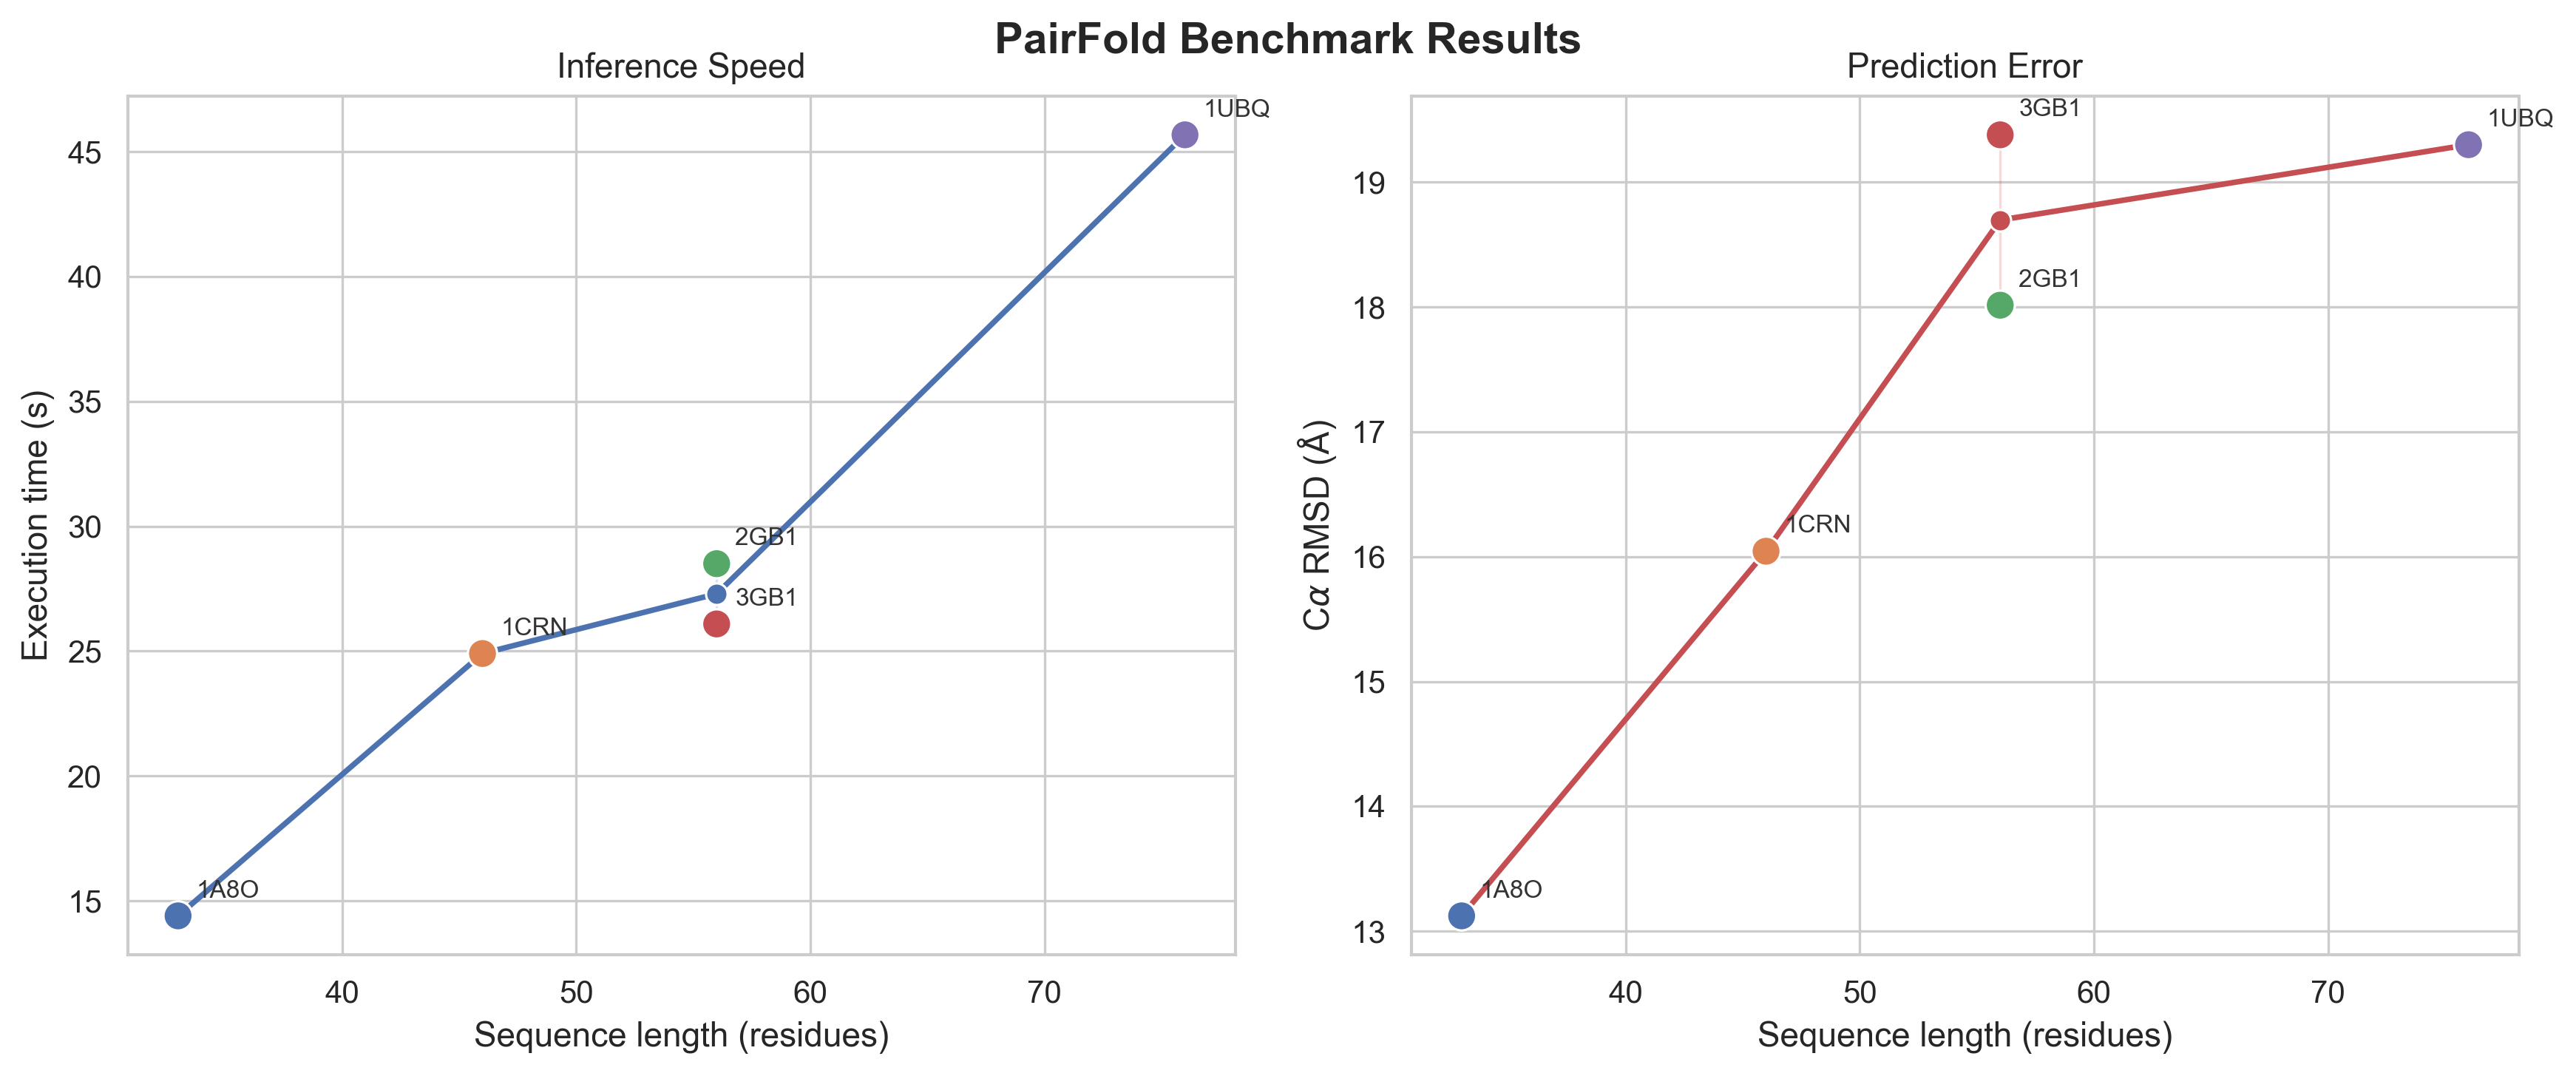
\includegraphics[width=\textwidth]{benchmark_plots.png}
  \caption{Paper-ready benchmark plots generated by \texttt{plot\_results.py}: (left) inference speed---sequence length versus execution time; (right) prediction error---sequence length versus C$\alpha$ RMSD. Points are annotated with PDB identifiers.}
  \label{fig:plots}
\end{figure}

\subsection{Speed--accuracy trade-off after look-ahead assembly}

Enabling clash-aware look-ahead backtracking, local $\phi/\psi$ relaxation, and post-SS lever polish changes the optimisation target from ``highest local confidence'' to ``locally clash-free and bend-plausible trajectories.''
Empirically:
\begin{itemize}[leftmargin=1.5em,itemsep=0.35em]
  \item \textbf{Speed.} Mean inference remains interactive on a consumer GPU ($27.9$\,s average across the five domains with contacts enabled; previously $5.89$\,s without the contact-conditioned hinge search). The additional cost is dominated by stronger anchor relaxation rather than the contact network forward pass.
  \item \textbf{Local geometry.} Soft clash energy and extreme lever over-extension are reduced; placements that would produce unphysical kinks are rejected or repaired before they propagate.
  \item \textbf{Global RMSD.} With \texttt{ContactPairNet} anchors enabled, mean Kabsch C$\alpha$ RMSD is $\approx 17.2$\,\AA\ (range $13.12$--$19.38$\,\AA), improving on the prior local-only mean of $18.50$\,\AA.
  Compact domains such as ubiquitin (1UBQ) improve substantially ($24.53{\to}19.30$\,\AA), while some small targets can move slightly away from the native basin when incorrect contacts compete with local geometry (e.g.\ 1CRN).
  Mean wall-clock increases to $\approx 28$\,s because contact-conditioned hinge search uses more Metropolis steps.
\end{itemize}

Thus the backtracking/relaxation stack is best interpreted as a \textbf{steric regulariser and lever mitigator}, not as a tertiary folding engine.
The observed trade-off is favourable when the scientific priority is fast, clash-aware backbone generation; it is insufficient when the priority is sub-$5$\,\AA\ global accuracy.

\subsection{Scaling behaviour}

At the angle level, PairFold accepts sequences up to $50\,000$ residues.
Full clash-aware assembly is limited to $N\le 256$; tertiary Metropolis refinement to $N\le 128$; tertiary score-only and atom export to $N\le 1000$.
These thresholds keep interactive use practical on consumer GPUs while preserving an $O(N)$ path for ultra-long visualisation.

% ===========================================================================
\section{Discussion}
% ===========================================================================

\subsection{What PairFold does well}

PairFold demonstrates that a small, PDB-trained fragment Transformer plus careful assembly can deliver:
(i)~interpretable $(\phi,\psi)$ predictions with calibrated confidence;
(ii)~secondary-structure-aware backbones;
(iii)~near-linear scaling for long sequences; and
(iv)~explicit handling of cumulative angular error via look-ahead and local torsion descent.
These properties suit teaching tools, rapid local design loops, and streaming visualisation---settings where AlphaFold's memory footprint is the bottleneck.

\subsection{Fundamental limitations}

The central limitation remains architectural relative to MSA-conditioned folding networks:
\texttt{ContactPairNet} is sequence-only and crop-trained, so contact precision is moderate (validation precision $\approx 0.18$ at the best checkpoint with high recall), and incorrect high-scoring pairs can pull the chain away from the native basin.
Without coevolutionary pair features or recycling, PairFold still cannot consistently reach sub-$5$\,\AA\ global accuracy on compact domains.
RMSD values of $13$--$19$\,\AA\ on $33$--$76$-residue domains should not be compared na\"ively to AlphaFold~2's typical low-\AA\ accuracy on the same targets~\citep{jumper2021alphafold}.

Additional limitations include:
\begin{itemize}[leftmargin=1.5em]
  \item Dependence on Chou--Fasman-style SS detection, which can misassign blocks on atypical sequences;
  \item Stochastic torsion relaxation that is not a true energy minimisation in a molecular force field;
  \item Contact anchors that are sparse and imperfect; hinge-based $\phi/\psi$ moves close distances only locally;
  \item Torsion training restricted to length $\le 5$, so medium-range motifs (e.g.\ $\beta$-turns spanning six residues) must emerge from assembly rather than from the torsion network.
\end{itemize}

\subsection{Future work}

Promising extensions that preserve PairFold's low-resource character include:
\begin{enumerate}[leftmargin=1.5em]
  \item Distilling PLM embeddings (e.g.\ small ESM-2) into the contact tower for higher precision without full MSA pipelines;
  \item Learning longer fragments ($6$--$9$-mers) or SE(3)-equivariant local frames while retaining DP segmentation;
  \item Using contact maps to rank assembly hypotheses earlier in look-ahead search, not only in post-hoc hinge relax;
  \item Systematic ablation of contact threshold, $k$, temperature $T$, and SS freezing on a larger PDB benchmark with confidence--RMSD calibration plots.
\end{enumerate}

% ===========================================================================
\section{Conclusion}
% ===========================================================================

We have presented PairFold, a complete local backbone generation system that couples a fragment Transformer on $(\phi,\psi)$ with $O(N)$ segmentation, temperature-calibrated confidence, secondary-structure freezing, look-ahead backtracking with lever-effect torsion relaxation, and a lightweight long-range \texttt{ContactPairNet}.
On five public domains, PairFold achieves mean inference time $27.9$\,s and mean C$\alpha$ RMSD $17.17$\,\AA\ (improved from $18.50$\,\AA\ without contacts), illustrating a clear regime: \textbf{fast, resource-light, locally plausible backbones with sparse tertiary restraints} rather than atomic-accuracy tertiary folds.
In an era dominated by large folding networks, such local alternatives remain scientifically and practically valuable---especially when sequences grow long, hardware is modest, and the question of interest is local geometry augmented by a cheap contact prior.

% ===========================================================================
\section*{Data and software availability}
% ===========================================================================

All software components described herein (\texttt{pairfold/predict.py}, \texttt{pairfold/clash\_assembly.py}, \texttt{pairfold/structure\_blocks.py}, \texttt{benchmark.py}, \texttt{plot\_results.py}) are part of the PairFold workspace.
Benchmark numbers are archived in \texttt{benchmark\_results.csv}; the figure is regenerated by \texttt{python plot\_results.py}.
Experimental structures were obtained from the RCSB PDB~\citep{berman2000protein}.

% ===========================================================================
\section*{Acknowledgements}
% ===========================================================================

The authors thank the open structural biology community for publicly deposited high-resolution crystal structures that make fragment-level supervision possible, and the developers of PyTorch, BioPython, and the scientific Python stack.

% ===========================================================================
\begin{thebibliography}{99}

\bibitem{jumper2021alphafold}
Jumper, J., Evans, R., Pritzel, A., et~al. (2021).
Highly accurate protein structure prediction with AlphaFold.
\textit{Nature}, 596, 583--589.
\url{https://doi.org/10.1038/s41586-021-03819-2}

\bibitem{senior2020alphafold}
Senior, A.~W., Evans, R., Jumper, J., et~al. (2020).
Improved protein structure prediction using potentials from deep learning.
\textit{Nature}, 577, 706--710.
\url{https://doi.org/10.1038/s41586-019-1923-7}

\bibitem{lin2023evolutionary}
Lin, Z., Akin, H., Rao, R., et~al. (2023).
Evolutionary-scale prediction of atomic-level protein structure with a language model.
\textit{Science}, 379, 1123--1130.
\url{https://doi.org/10.1126/science.ade2574}

\bibitem{simons1997assembly}
Simons, K.~T., Kooperberg, C., Huang, E., \& Baker, D. (1997).
Assembly of protein tertiary structures from fragments with similar local sequences using simulated annealing and Bayesian scoring functions.
\textit{Journal of Molecular Biology}, 268, 209--225.
\url{https://doi.org/10.1006/jmbi.1997.0959}

\bibitem{rohl2004rosetta}
Rohl, C.~A., Strauss, C.~E.~M., Misura, K.~M.~S., \& Baker, D. (2004).
Protein structure prediction using Rosetta.
\textit{Methods in Enzymology}, 383, 66--93.
\url{https://doi.org/10.1016/S0076-6879(04)83004-0}

\bibitem{ramachandran1963stereochemistry}
Ramachandran, G.~N., Ramakrishnan, C., \& Sasisekharan, V. (1963).
Stereochemistry of polypeptide chain configurations.
\textit{Journal of Molecular Biology}, 7, 95--99.
\url{https://doi.org/10.1016/S0022-2836(63)80023-6}

\bibitem{engh1991accurate}
Engh, R.~A., \& Huber, R. (1991).
Accurate bond and angle parameters for X-ray protein structure refinement.
\textit{Acta Crystallographica Section A}, 47, 392--400.
\url{https://doi.org/10.1107/S0108767391001071}

\bibitem{berens2009circ}
Berens, P. (2009).
CircStat: A MATLAB toolbox for circular statistics.
\textit{Journal of Statistical Software}, 31, 1--21.
\url{https://doi.org/10.18637/jss.v031.i10}

\bibitem{chou1974prediction}
Chou, P.~Y., \& Fasman, G.~D. (1974).
Prediction of protein conformation.
\textit{Biochemistry}, 13, 222--245.
\url{https://doi.org/10.1021/bi00699a002}

\bibitem{berman2000protein}
Berman, H.~M., Westbrook, J., Feng, Z., et~al. (2000).
The Protein Data Bank.
\textit{Nucleic Acids Research}, 28, 235--242.
\url{https://doi.org/10.1093/nar/28.1.235}

\end{thebibliography}

\end{document}
